\documentclass[11pt]{article}
\usepackage[preprint]{acl}
\usepackage{times}
\usepackage{latexsym}
\usepackage[T1]{fontenc}
\usepackage[utf8]{inputenc}
\usepackage{microtype}
\usepackage{lmodern}
\renewcommand{\ttdefault}{lmtt}
\renewcommand{\rmdefault}{ptm}
\renewcommand{\sfdefault}{phv}
\usepackage{graphicx}
\usepackage{booktabs}
\usepackage{adjustbox}
\usepackage{tabularx}
\usepackage{array}
\usepackage{enumitem}
\usepackage{newunicodechar}
\usepackage{morefloats}
\usepackage[section]{placeins}
\extrafloats{200}
\renewcommand{\topfraction}{0.95}
\renewcommand{\dbltopfraction}{0.95}
\renewcommand{\textfraction}{0.05}
\renewcommand{\floatpagefraction}{0.6}
\renewcommand{\dblfloatpagefraction}{0.6}
\setcounter{topnumber}{4}
\setcounter{dbltopnumber}{4}
\usepackage{tikz}
\usetikzlibrary{positioning,arrows.meta,calc}

\newunicodechar{−}{\ensuremath{-}}
\newunicodechar{×}{\ensuremath{\times}}
\newunicodechar{÷}{\ensuremath{\div}}
\newunicodechar{→}{\ensuremath{\rightarrow}}
\newunicodechar{≥}{\ensuremath{\geq}}
\newunicodechar{≤}{\ensuremath{\leq}}
\newunicodechar{≈}{\ensuremath{\approx}}
\newunicodechar{…}{\ldots}
\newunicodechar{·}{\ensuremath{\cdot}}
\newunicodechar{‑}{-}

\providecommand{\tightlist}{\setlength{\itemsep}{0pt}\setlength{\parskip}{0pt}}
\setlist{nosep,leftmargin=*}
\emergencystretch=3em
\hbadness=10000
\hfuzz=20pt
\setcounter{secnumdepth}{3}

\title{Intent-Gated Data Transformation Agent: Final Report}
\author{\textbf{Team SSSS} $\cdot$ LMA Group Project 2026 \\[4pt]
  Akash Sigullapalli (2023101104) \quad Konapalli Jaswanth Reddy (2023101025) \\
  Kotha Sai Veekshith (2023101078) \quad Srinivas Billuri (2023101029)}

\begin{document}
\maketitle
\begin{abstract}
Large language models (LLMs) are often used to write data-transformation
code from natural-language requests. Such code can run without error but
silently do the wrong thing, for example by removing valid rows or
changing columns the user did not mention. Conventional data-quality
checks cannot reliably catch these errors, because they do not know what
the user asked for.

We propose an \textbf{intent-gated} pipeline. A parser turns each
request into an \textbf{intent contract}: a short list of checkable
statements stating what the transformation \emph{must change} and what
it \emph{must preserve}. After the generated code runs in a sandbox, a
deterministic verifier checks the data before and after against the
contract, and a bounded, tool-using repair agent tries to fix code that
fails.

We built a benchmark of 120 tasks on four public datasets and a frozen
pool of 803 LLM-written programs labelled correct or wrong. With gold
contracts, the verifier catches 94.4\% of silently wrong programs with
no false rejections, against 45.5\% recall and 13.9\% false rejection
for conventional checks. A QLoRA fine-tuned Qwen2.5-1.5B parser writes
better contracts than a prompted Qwen2.5-7B model (2\% vs 13\% invalid
contracts). Two later 1.5B parsers, which receive the data statistics a
request needs, lower the false-rejection rate further to 0.120 and
0.139.

End to end on 100 test tasks, the best system, which uses a 3B repair
agent guided by repair hints, gives 82 correct outputs with 2 wrong
outputs accepted, against 78 correct and 20 wrong for direct generation
and 75 correct and 11 wrong for conventional checks with the same repair
agent. The reduction in wrong outputs is large, while the gain in
correct outputs is not statistically significant. With gold contracts
the same system solves 92 of 100 tasks, which shows that contract
quality is the main bottleneck. No unsafe code was executed in any run.

\end{abstract}

\section{Introduction}

\subsection{Motivation}

Data preparation includes filtering rows, removing duplicates, handling
missing values, converting types and deriving new columns. It is now
common to ask an LLM to write this code from a short request such as
"remove passengers younger than 18; unknown ages stay".

The main risk is not code that crashes, because a crash is visible. The
risk is code that \textbf{runs successfully but does the wrong thing}.
In our candidate pool, about a third of the distinct programs that run
are silently wrong. Typical mistakes are removing extra rows,
deduplicating on the wrong key, filling missing values in every column,
converting to the wrong type, and leaving helper columns in the output.

Generic data-quality checks, such as row counts, null counts and
distribution shifts, \textbf{do not know the user's intent}. A correct
filter that removes 20\% of the rows looks the same as a faulty one that
removes 20\% by mistake.

\subsection{Our approach}

For each request, an \textbf{intent parser} writes an \textbf{intent
contract} in a closed vocabulary of 11 predicate types. The contract has
two halves:

\begin{itemize}
\tightlist
\item
  \textbf{\texttt{must\_\allowbreak{}change}} states what the request
  asks to change, e.g. "every row with Age \textless{} 18 is removed".
\item
  \textbf{\texttt{must\_\allowbreak{}preserve}} states what should stay
  the same even though the user did not say so, e.g. "every row with Age
  ≥ 18 or unknown Age is kept, and no column changes".
\end{itemize}

A \textbf{deterministic verifier} checks every predicate against the
data before and after; no LLM is used as a judge. If the check fails, a
\textbf{repair agent} reads the failure report, may inspect the data
with read-only tools, and proposes revised code within a fixed budget. A
static safety checker blocks unsafe code before it runs. The project
therefore combines \textbf{fine-tuning} (the parser), \textbf{tool
calling} (the repair agent) and \textbf{agentic behaviour} (repairing,
inspecting or escalating to a human).

\subsection{Research question and hypotheses}

\textbf{Research question.} Does an intent contract that specifies what
must change and what must be preserved improve the detection of silent
semantic errors in LLM-generated data transformations, and does an agent
that combines such contracts with an intent parser and a repair loop
increase the accuracy of data transformations?

\begin{table*}[!tp]
\centering\footnotesize\setlength{\tabcolsep}{3pt}\renewcommand{\arraystretch}{1.1}
\begin{tabularx}{\textwidth}{l>{\raggedright\arraybackslash}X>{\raggedright\arraybackslash}X}
\toprule
\textbf{Part} & \textbf{Question} & \textbf{Evaluated in} \\
\midrule
RQ1: detection & Do intent contracts detect silent errors better than conventional checks? & Stage 1: all systems judge the same frozen pool of programs \\
RQ2: accuracy & Does the full agent deliver more correct transformations than direct generation? & Stage 2: the full pipeline runs end to end on 100 test tasks \\
\bottomrule
\end{tabularx}
\end{table*}

\begin{itemize}
\tightlist
\item
  \textbf{H1:} intent-based verification accepts fewer wrong
  transformations than conventional checks while keeping false
  rejections low.
\item
  \textbf{H2:} the intent-gated agent with repair delivers more correct
  accepted outputs than direct generation.
\end{itemize}

\section{Literature Review}

\textbf{LLM code generation for data science.} Codex and HumanEval (Chen
et al., 2021) made functional correctness against tests the standard
evaluation. DS-1000 (Lai et al., 2023) and Jigsaw (Jain et al., 2022)
study data-science and pandas code. These benchmarks need
\textbf{reference outputs}, which do not exist in a real deployment. Our
work judges a transformation using only the request and the data.

\textbf{Data validation.} Deequ (Schelter et al., 2018), TensorFlow data
validation (Breck et al., 2019), Great Expectations and Pandera
(Bantilan, 2020) check \textbf{generic, request-independent} properties.
Our conventional baseline follows this family. Our contracts can be seen
as data tests generated \textbf{per request}, in two directions.

\textbf{Specifications for generated code.} Our contracts follow
\textbf{design by contract} (Meyer, 1992). nl2postcond (Endres et al.,
2024) and nl2spec (Cosler et al., 2023) use LLMs to write
specifications, and CodeT (Chen et al., 2023) uses generated tests to
select programs. These studies show that generated specifications can be
wrong. We add a closed vocabulary, an explicit must-preserve half and a
deterministic verifier.

\textbf{Self-repair and tool-using agents.} Self-Refine (Madaan et al.,
2023), Self-Debugging (Chen et al., 2024), Reflexion (Shinn et al.,
2023), ReAct (Yao et al., 2023) and Toolformer (Schick et al., 2023) let
models improve output with feedback and tools. Our repair agent works
under a \textbf{fixed external judge}: the verifier, not the model,
decides whether a fix is accepted, and the contract is read-only.

\textbf{Efficient fine-tuning.} LoRA (Hu et al., 2022) and QLoRA
(Dettmers et al., 2023) make fine-tuning possible on a single small GPU.
We use QLoRA on Qwen2.5 models (Qwen Team, 2024) with plain greedy
decoding and strict schema validation, without constrained decoding
(Willard and Louf, 2023).

\textbf{Gap.} To our knowledge, no earlier system writes a
request-specific, two-sided contract for a tabular transformation,
checks it without a reference output, uses it to drive a bounded repair
agent, and is evaluated both for error detection and for end-to-end
accuracy.

\section{Dataset Created / Used}

\begin{table*}[!tp]
\centering\footnotesize\setlength{\tabcolsep}{3pt}\renewcommand{\arraystretch}{1.1}
\begin{tabularx}{\textwidth}{l>{\raggedright\arraybackslash}X}
\toprule
\textbf{Material} & \textbf{Content} \\
\midrule
Evaluation datasets & Four public tables: UCI Adult (1,000 × 15), NYC Airbnb 2019 (1,000 × 16), Titanic (891 × 12), NYC Yellow Taxi January 2026 (1,000 × 20) \\
Task set & 120 tasks = 4 datasets × 5 types × 6 tasks (filtering, deduplication, missing values, type conversion, column transformation); 100 test and 20 dev tasks \\
Candidate pool & 803 distinct programs from Qwen2.5-3B and 1.5B (1 greedy + 5 sampled per task); test split: 630 runnable, 213 wrong, 417 correct \\
Agent scenarios & 222 test scenarios: repairable (82), already correct (95), tool fault (24), should escalate (12), safety (9) \\
Red-team set & 27 unsafe programs (file, network, shell, process, code execution, interpreter escapes, resource exhaustion) \\
Fine-tuning corpus & 3,614 training and 796 validation examples on 8 datasets that never appear in evaluation \\
\bottomrule
\end{tabularx}
\end{table*}

\textbf{Tasks.} Each task has a natural-language request, a correct
\texttt{reference\_\allowbreak{}code}, a
\texttt{gold\_\allowbreak{}contract} and the expected effect. Requests
never state what must be preserved; the gold contract adds it with a
default-preservation rule (rows not targeted are kept, columns not
mentioned are unchanged). Every contract must fail for each plausible
wrong reading of the request, such as a shifted boundary or a wrong
deduplication key.

\textbf{Labelling.} Every program runs in the sandbox, and its output is
compared with the reference output by content (same columns, rows, dtype
families and values). Equal outputs are labelled correct, all others
wrong. All errors in the pool were therefore made by language models,
not written by hand.

\textbf{Fine-tuning corpus.} Examples were generated from 43 patterns
that cover all predicates and functions. An automatic checker kept an
example only if its contract is valid, its reference passes, a no-op
fails, and its request does not overlap with evaluation requests. A hand
review of 100 examples found 99 correct.

\section{Methodology}

\subsection{System overview}
\begin{figure*}[t]
\centering\scriptsize
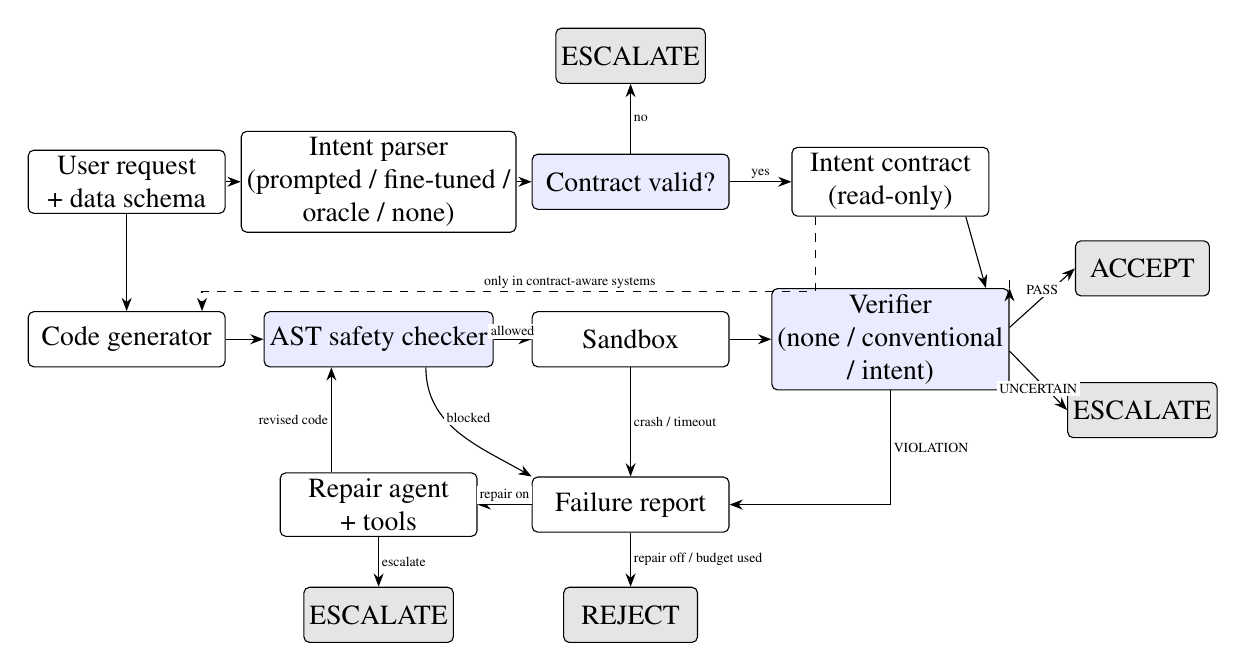
\begin{tikzpicture}[
  node distance=0pt, >=Stealth,
  box/.style={draw, rounded corners=2pt, minimum width=2.5cm, minimum height=0.7cm, align=center, inner sep=2pt, fill=white},
  term/.style={box, fill=gray!20, minimum width=1.7cm},
  dec/.style={box, fill=blue!8},
  lab/.style={font=\tiny, fill=white, inner sep=1pt}]
% row A
\node[box] (req) at (1.3,2) {User request\\+ data schema};
\node[box] (par) at (4.5,2) {Intent parser\\(prompted / fine-tuned /\\oracle / none)};
\node[dec] (val) at (7.7,2) {Contract valid?};
\node[box] (con) at (11.0,2) {Intent contract\\(read-only)};
\node[term] (esc1) at (7.7,3.6) {ESCALATE};
% row B
\node[box] (gen) at (1.3,0) {Code generator};
\node[dec] (saf) at (4.5,0) {AST safety checker};
\node[box] (sbx) at (7.7,0) {Sandbox};
\node[dec] (ver) at (11.0,0) {Verifier\\(none / conventional\\/ intent)};
\node[term] (acc) at (14.2,0.9) {ACCEPT};
\node[term] (esc2) at (14.2,-0.9) {ESCALATE};
% row C
\node[box] (rep) at (4.5,-2.1) {Repair agent\\+ tools};
\node[box] (fr) at (7.7,-2.1) {Failure report};
\node[term] (rej) at (7.7,-3.5) {REJECT};
\node[term] (esc3) at (4.5,-3.5) {ESCALATE};
% edges
\draw[->] (req) -- (par);
\draw[->] (par) -- (val);
\draw[->] (val) -- node[lab,above]{yes} (con);
\draw[->] (val) -- node[lab,right]{no} (esc1);
\draw[->] (req.south) -- (gen.north);
\draw[->,dashed] ($(con.south west)+(0.3,0)$) -- ++(0,-0.95) -| node[lab,pos=0.2,above]{only in contract-aware systems} ($(gen.north east)+(-0.3,0)$);
\draw[->] ($(con.south east)+(-0.3,0)$) -- ($(ver.north east)+(-0.3,0)$);
\draw[->] (gen) -- (saf);
\draw[->] (saf) -- node[lab,above]{allowed} (sbx);
\draw[->] (sbx) -- (ver);
\draw[->] (ver.north east) ++(0,0) -- ++(0,0) coordinate (x);
\draw[->] ($(ver.east)+(0,0.15)$) -- node[lab,above,pos=0.5]{PASS} (acc.west);
\draw[->] ($(ver.east)+(0,-0.15)$) -- node[lab,below,pos=0.5]{UNCERTAIN} (esc2.west);
\draw[->] (ver.south) |- node[lab,pos=0.25,right]{VIOLATION} (fr.east);
\draw[->] (sbx.south) -- node[lab,right]{crash / timeout} (fr.north);
\draw[->] ($(saf.south)+(0.6,0)$) to[out=-90,in=150] node[lab,pos=0.35,right]{blocked} (fr.north west);
\draw[->] (fr) -- node[lab,above]{repair on} (rep);
\draw[->] (fr) -- node[lab,right]{repair off / budget used} (rej);
\draw[->] ($(rep.north)+(-0.6,0)$) -- node[lab,left]{revised code} ($(saf.south)+(-0.6,0)$);
\draw[->] (rep) -- node[lab,right]{escalate} (esc3);
\end{tikzpicture}
\caption{System overview.}
\label{fig:overview}
\end{figure*}




Every system in this report is a configuration of the same parts.
Systems differ in the parser, the verifier, whether the generator sees
the contract, and whether repair is enabled. Every run ends as
\textbf{ACCEPT}, \textbf{REJECT} or \textbf{ESCALATE}.

\subsection{Intent contracts and verifier}

A contract is a JSON object with a \texttt{must\_\allowbreak{}change}
list and a \texttt{must\_\allowbreak{}preserve} list, built from 11
predicate types:

\begin{table*}[!tp]
\centering\footnotesize\setlength{\tabcolsep}{3pt}\renewcommand{\arraystretch}{1.1}
\begin{tabularx}{\textwidth}{l>{\raggedright\arraybackslash}X}
\toprule
\textbf{Predicate group} & \textbf{Predicates} \\
\midrule
Rows & \texttt{row\_\allowbreak{}count}, \texttt{rows\_\allowbreak{}removed\_\allowbreak{}where}, \texttt{rows\_\allowbreak{}retained\_\allowbreak{}where}, \texttt{duplicate\_\allowbreak{}count} (with a keep rule) \\
Values & \texttt{null\_\allowbreak{}count}, \texttt{column\_\allowbreak{}values\_\allowbreak{}unchanged}, \texttt{column\_\allowbreak{}value\_\allowbreak{}relation} (14 functions, e.g. \texttt{sub}, \texttt{clip}, \texttt{map}, \texttt{cast}) \\
Columns & \texttt{columns\_\allowbreak{}unchanged}, \texttt{column\_\allowbreak{}dtype}, \texttt{columns\_\allowbreak{}added}, \texttt{columns\_\allowbreak{}removed} \\
\bottomrule
\end{tabularx}
\end{table*}

Contracts are validated strictly; an invalid contract leads to
escalation. The \textbf{verifier} uses no language model. It aligns rows
by index (or by content if the index was lost), checks each predicate,
and returns VIOLATION if any predicate fails, UNCERTAIN if one cannot be
evaluated, and PASS otherwise. Each failure is reported with expected
and observed values and example rows.

\subsection{Safety checker and sandbox}

An AST checker allows only \texttt{pandas} and \texttt{numpy} imports
and blocks file, network, shell and code-execution calls. Code runs in
an isolated interpreter in an empty temporary directory, with limits on
CPU time, memory and output size.

\subsection{Code generator}

The generator is Qwen2.5-3B-Instruct. Prompt \texttt{b1-v1} gives the
request and the schema (column names, dtypes, missing counts, first 5
rows). Prompt \texttt{b2-v2} adds the contract and general
implementation rules.

\subsection{Intent parsers}

All parsers use greedy decoding followed by strict schema validation,
with no output repair.

\begin{table*}[!tp]
\centering\footnotesize\setlength{\tabcolsep}{3pt}\renewcommand{\arraystretch}{1.1}
\begin{tabularx}{\textwidth}{l>{\raggedright\arraybackslash}X}
\toprule
\textbf{Parser} & \textbf{Description} \\
\midrule
Prompted (Baseline 3) & Qwen2.5-7B with vocabulary description, a reference card and five dev examples; prompt version chosen on dev only \\
Fine-tuned & Qwen2.5-1.5B and 3B trained with QLoRA (4-bit NF4, LoRA rank 16, alpha 32, 2 epochs, loss on contract tokens) \\
Selective facts & 1.5B adapter (4,003 examples). A rule-based program computes the statistics the request needs (median, mean or mode of a column or group) and adds them to the input \\
Tool use & 1.5B adapter (4,743 conversations). The parser calls read-only data tools, such as \texttt{profile\_\allowbreak{}column}, to get the facts itself \\
Oracle & Returns the gold contract; an upper bound, not a deployable system \\
\bottomrule
\end{tabularx}
\end{table*}

The two later parsers were trained because the first fine-tuned parser
had to guess statistics it could not see. In Config 2 they also use a
\textbf{contract self-check}: simple checks on the input table look for
unknown columns, filter values that match no row and deduplication keys
without duplicates, and the parser may correct the contract once.

\subsection{Conventional checks (Baseline 2)}

A generic data-quality suite compares only the input and output tables,
never the request. It measures schema, row, null, dtype, uniqueness,
range and distribution changes. Thresholds were tuned on the dev split
to maximise recall with at most 10\% false rejection.

\subsection{Repair agent}

In each step the agent either calls a tool
(\texttt{inspect\_\allowbreak{}dataset},
\texttt{profile\_\allowbreak{}column},
\texttt{diff\_\allowbreak{}datasets},
\texttt{run\_\allowbreak{}transformation},
\texttt{run\_\allowbreak{}verifier}), proposes new code, or escalates.
It never sees gold contracts or reference outputs. Limits are 3 repair
attempts, 8 tool calls per attempt and 60,000 tokens per task; proposing
identical code twice leads to escalation.

Two repair configurations are used in Stage 2:

\begin{table*}[!tp]
\centering\footnotesize\setlength{\tabcolsep}{3pt}\renewcommand{\arraystretch}{1.1}
\begin{tabularx}{\textwidth}{l>{\raggedright\arraybackslash}X>{\raggedright\arraybackslash}X}
\toprule
\textbf{} & \textbf{Config 1} & \textbf{Config 2} \\
\midrule
Repair model & Qwen2.5-7B, 4-bit & Qwen2.5-3B, FP16 \\
Repair prompt & Failure report, tools, memory of earlier attempts & Same, plus a short attempt history, a fresh recovery request, a schema guard against undeclared columns, and repair hints \\
Parsers used with it & First fine-tuned 1.5B & Selective-facts and tool-use 1.5B, with the contract self-check \\
\bottomrule
\end{tabularx}
\end{table*}

The repair hints add pandas code lines for each failed predicate and
warnings for common mistakes, such as sorting before
\texttt{drop\_\allowbreak{}duplicates} or using \texttt{dropna} when it
was not requested. Systems without a contract (Baseline 2) use Config 2
without the parts that need a contract: no contract text, no schema
guard and no hints.

\subsection{Evaluation design and metrics}

\textbf{Stage 1} applies every verifier to the same frozen pool, so
comparisons are paired. \textbf{Stage 2} runs the full pipeline live on
the 100 test tasks with greedy decoding and seed 0. Outputs are compared
with the reference only offline, after the run.

\begin{table*}[!tp]
\centering\footnotesize\setlength{\tabcolsep}{3pt}\renewcommand{\arraystretch}{1.1}
\begin{tabularx}{\textwidth}{l>{\raggedright\arraybackslash}X}
\toprule
\textbf{Metric} & \textbf{Definition} \\
\midrule
Recall & Wrong candidates not accepted ÷ runnable wrong candidates \\
False-rejection rate (FRR) & Correct candidates not accepted ÷ correct candidates \\
Silent error rate & Wrong accepted ÷ all accepted \\
Invalid rate, exact match, F1 & Contract quality against the gold contract \\
Final accuracy & The final output was accepted and equals the reference \\
\bottomrule
\end{tabularx}
\end{table*}

Paired comparisons use the exact McNemar test.

\section{Experiment Runs}

\begin{table*}[!tp]
\centering\footnotesize\setlength{\tabcolsep}{3pt}\renewcommand{\arraystretch}{1.1}
\begin{tabularx}{\textwidth}{l>{\raggedright\arraybackslash}Xl>{\raggedright\arraybackslash}X}
\toprule
\textbf{\#} & \textbf{Experiment} & \textbf{Stage} & \textbf{Main result (test)} \\
\midrule
1 & Baseline 1: direct LLM, no verification & 1 & Greedy accuracy 77/100 (3B); silent error rate 0.338 \\
2 & Baseline 2: conventional checks & 1 & Recall 0.455, FRR 0.139 \\
3 & Oracle: gold contracts & 1 & Recall 0.944, FRR 0.000 \\
4 & Baseline 3: prompted 7B parser & 1 & Recall 0.892, FRR 0.254; 13\% invalid contracts \\
5 & Agent evaluation on agent scenarios & Agent & Full agent repaired 58/82; 0 unsafe executions \\
6 & Fine-tuned parsers (1.5B, 3B) & 1 & Recall 0.944 / 0.915, FRR 0.165 / 0.158; 2\% invalid \\
6b & Selective-facts and tool-use parsers & 1 & Recall 0.944 / 0.930, FRR 0.120 / 0.139 \\
7 & Stage 2 with Config 1 (7B repair) & 2 & Direct 78 correct (20 wrong accepted); proposed 76 (2) \\
7b & Stage 2 with Config 2 (3B repair + hints) & 2 & Proposed 82 (2) and 80 (1); Baseline 2 + repair 75 (11); gold 92 (0) \\
8 & Safety evaluation & All & 27/27 red-team programs blocked or contained \\
\bottomrule
\end{tabularx}
\end{table*}

\textbf{Experiment 1} measures the problem. Even with greedy decoding
the 3B generator solves about one task in four wrongly, and
deduplication is the most error-prone type (silent error rate 0.556).

\textbf{Experiment 2} tests a tuned conventional baseline. Its
mean-shift check causes all of its false rejections, because correct
filters and deduplications also shift column means. It catches no
type-conversion errors.

\textbf{Experiment 3} tests the core idea with gold contracts. It
catches almost all errors; its 12 misses come from known vocabulary gaps
(helper columns and one unconstrained dtype).

\textbf{Experiment 4} shows intent verification with imperfect
contracts. Of the prompted parser's 106 false rejections, 51 come from
invalid contracts and 55 from wrongly written predicates.

\textbf{Experiment 5} compares the full repair agent with two simpler
retry strategies on 222 agent scenarios. All use Qwen2.5-7B and gold
contracts.

\textbf{Experiments 6 and 6b} test whether a small fine-tuned parser can
replace the prompted 7B parser, and whether giving it the needed
statistics helps further.

\textbf{Experiment 7} runs the full pipeline end to end with Config 1
(first fine-tuned parser, 7B repair agent). \textbf{Experiment 7b}
repeats it with Config 2 (newer parsers, contract self-check, 3B repair
agent with hints). In Config 2, Baseline 2 + repair and the
no-contract-to-generator ablation were run again with the same 3B
generator and repair model. Baselines 1 and 3 were not run again.

\textbf{Experiment 8} sends every red-team program through every
execution path and counts unsafe attempts in all real runs.

\section{Ablation Studies}

Each ablation changes one part of a system and keeps everything else
fixed.

\begin{table*}[!tp]
\centering\footnotesize\setlength{\tabcolsep}{3pt}\renewcommand{\arraystretch}{1.1}
\begin{tabularx}{\textwidth}{l>{\raggedright\arraybackslash}X>{\raggedright\arraybackslash}X}
\toprule
\textbf{\#} & \textbf{Ablation} & \textbf{Result} \\
\midrule
A1 & Contract direction (gold contracts) & Full contract recall 0.944; change-only 0.732; preserve-only 0.446. Both halves are needed \\
A2 & Prompted parser size & FRR: 7B 0.254, 3B 0.578, 1.5B 0.796. Small prompted parsers reach high recall only by rejecting almost everything \\
A3 & Fine-tuning vs prompting at 1.5B & Invalid 0.34 → 0.02; FRR 0.796 → 0.165 \\
A4 & Prompt version (7B) & Invalid contracts 0.34 → 0.33 → 0.13 from p1-v1 to p1-v3 \\
A5 & Baseline 2 thresholds & Stricter thresholds raise recall to 0.742 but FRR to 0.561 \\
A6 & Generator model & Greedy accuracy 77 (3B) vs 76 (1.5B); the 1.5B model produces more errors when sampling \\
A7 & Repair strategy & R repaired: naive 50, feedback 51, full agent 58 of 82 (not significant; about 5 times more tokens) \\
A8 & Effect of repair (Config 1) & Repair gain +0.10 for the proposed system and +0.17 with gold contracts \\
A9 & Contract given to the generator & Config 1: 76 vs 73 correct (p = 0.508). Config 2: 82 vs 79 (selective facts, p = 0.375) and 80 vs 78 (tool use, p = 0.727). A small, non-significant benefit \\
A10 & Gold contract (Config 1) & 94 vs 76 correct (p < 0.001) \\
\bottomrule
\end{tabularx}
\end{table*}

The most important findings are A1 and A3.
\texttt{must\_\allowbreak{}change} alone misses code that removes the
right rows \emph{and} extra ones, because "these rows are gone" still
holds. \texttt{must\_\allowbreak{}preserve} alone cannot see that a
requested change did not happen. Fine-tuning, not model size, makes a
small parser produce valid contracts: a fine-tuned 1.5B parser beats a
prompted 7B parser.

\section{Evaluations}

\subsection{Stage 1: verification on the frozen pool}

Test split, 671 candidates (213 runnable wrong, 417 correct). Brackets
give 95\% bootstrap intervals.

\begin{table*}[!tp]
\centering\footnotesize\setlength{\tabcolsep}{3pt}\renewcommand{\arraystretch}{1.1}
\begin{tabularx}{\textwidth}{>{\raggedright\arraybackslash}Xllll}
\toprule
\textbf{System} & \textbf{Invalid} & \textbf{Recall} & \textbf{FRR} & \textbf{Silent error rate} \\
\midrule
Baseline 1: no verification & — & 0.000 & 0.000 & 0.338 \\
Baseline 2: conventional checks & — & 0.455 [0.33, 0.58] & 0.139 [0.07, 0.22] & 0.244 \\
Baseline 3: prompted 7B & 13\% & 0.892 [0.82, 0.95] & 0.254 [0.16, 0.36] & 0.069 \\
Fine-tuned 1.5B & 2\% & 0.944 [0.90, 0.98] & 0.165 [0.09, 0.25] & 0.033 \\
Fine-tuned 3B & 2\% & 0.915 [0.85, 0.97] & 0.158 [0.09, 0.24] & 0.049 \\
Selective-facts 1.5B & 5\% & \textbf{0.944} [0.90, 0.98] & \textbf{0.120} [0.06, 0.20] & 0.032 \\
Tool-use 1.5B & 1\% & 0.930 [0.88, 0.97] & 0.139 [0.07, 0.22] & 0.040 \\
Oracle (gold contracts) & 0\% & 0.944 [0.90, 0.98] & 0.000 & 0.028 \\
\bottomrule
\end{tabularx}
\end{table*}

All intent-based systems are significantly better than conventional
checks (McNemar p \textless{} 0.005). Both first fine-tuned parsers are
significantly better than the prompted 7B parser (p \textless{} 0.001),
and the two sizes do not differ (p = 0.822). The selective-facts parser
is significantly better than the first fine-tuned 1.5B parser (40 vs 21
candidates, p = 0.020); the tool-use parser is not (p = 0.382). The two
newer parsers were scored from the contracts they wrote in Stage 2 runs
and developed after earlier test results were known, so their rows are
exploratory.

\textbf{By type}, conventional checks catch no type-conversion errors (0
of 29) and reject 49\% of correct deduplications. The gold contracts
catch all 29 type-conversion errors. Contract quality is still weakest
for type conversion (exact match 10--20\% for all fine-tuned parsers),
because ordered categories and datetime conversions are rare in the
training data.

\subsection{Agent evaluation}

222 test scenarios, Qwen2.5-7B, gold contracts, seed 0. Three repair
strategies are compared:

\begin{itemize}
\tightlist
\item
  \textbf{Full agent:} the agent receives the failure report, can call
  data-inspection tools, remembers its earlier attempts, and can choose
  to escalate.
\item
  \textbf{Feedback retry:} the model simply writes new code. It sees the
  previous code and the failure report, but has no tools and no memory
  beyond the last attempt.
\item
  \textbf{Naive retry:} the model writes new code after being told only
  that "verification failed", with no information about what went wrong.
\end{itemize}

Brackets give 95\% Wilson intervals.

\begin{table*}[!tp]
\centering\footnotesize\setlength{\tabcolsep}{3pt}\renewcommand{\arraystretch}{1.1}
\begin{tabularx}{\textwidth}{l>{\raggedright\arraybackslash}Xlll}
\toprule
\textbf{Scenario kind} & \textbf{Measure} & \textbf{Full agent} & \textbf{Feedback retry} & \textbf{Naive retry} \\
\midrule
R (82) & Repaired & \textbf{58 (0.71)} [0.60, 0.80] & 51 (0.62) & 50 (0.61) \\
C (95) & Correct code accepted with no action & 95 & 95 & 95 \\
T (24) & Repaired despite a tool fault & \textbf{18} & 15 & 16 \\
E (12) & Escalated / rejected / accepted & 8 / 4 / 0 & 10 / 2 / 0 & 12 / 0 / 0 \\
S (9) & Accepted (safe part only) / escalated / rejected & 7 / 1 / 1 & 4 / 4 / 1 & 2 / 6 / 1 \\
All & Unsafe code executed & \textbf{0} & \textbf{0} & \textbf{0} \\
\bottomrule
\end{tabularx}
\end{table*}

The full agent repairs the most code, recovers from 18 of 24 injected
tool faults, and never accepts an impossible request. Its advantage over
the simpler strategies is not significant (p ≥ 0.17), and it uses about
5 to 6 times as many tokens. On unsafe requests the agent completes only
the safe part instead of refusing.

\subsection{Stage 2: end-to-end evaluation}

100 test tasks, generator Qwen2.5-3B, greedy decoding. Final accuracy
counts a task only if a correct output was accepted. Each repair
configuration is described in the Methodology section.

\begin{table*}[!tp]
\centering\footnotesize\setlength{\tabcolsep}{3pt}\renewcommand{\arraystretch}{1.1}
\begin{tabularx}{\textwidth}{>{\raggedright\arraybackslash}Xlllll}
\toprule
\textbf{System} & \textbf{Parser} & \textbf{Correct} & \textbf{Wrong accepted} & \textbf{Withheld} & \textbf{Accepted-output correctness} \\
\midrule
Baseline 1 (direct, no repair) & none & 78 & 20 & 2 & 79.6\% \\
\emph{Config 1: 7B repair agent} &  &  &  &  &  \\
Baseline 2 + repair & none & 72 & 13 & 15 & 84.7\% \\
Baseline 3 + repair & prompted 7B & 67 & 3 & 30 & 95.7\% \\
Proposed & fine-tuned 1.5B & 76 & 2 & 22 & 97.4\% \\
No contract to generator & fine-tuned 1.5B & 73 & 2 & 25 & 97.3\% \\
Gold contract & oracle & 94 & 0 & 6 & 100\% \\
\emph{Config 2: 3B repair agent + hints} &  &  &  &  &  \\
Baseline 2 + repair & none & 75 & 11 & 14 & 87.2\% \\
\textbf{Proposed (selective facts)} & selective-facts 1.5B & \textbf{82} & 2 & 16 & 97.6\% \\
\textbf{Proposed (tool use)} & tool-use 1.5B & 80 & \textbf{1} & 19 & \textbf{98.8\%} \\
No contract to generator (selective facts) & selective-facts 1.5B & 79 & 2 & 19 & 97.5\% \\
No contract to generator (tool use) & tool-use 1.5B & 78 & 1 & 21 & 98.7\% \\
Gold contract & oracle & 92 & 0 & 8 & 100\% \\
\bottomrule
\end{tabularx}
\end{table*}

Paired comparisons (exact McNemar) of the Config 2 proposed systems:
against direct generation, selective facts 12 vs 8 tasks (p = 0.503) and
tool use 14 vs 12 (p = 0.845); against Baseline 2 + repair in Config 2,
selective facts 14 vs 7 (p = 0.189) and tool use 16 vs 11 (p = 0.442).
Gold contracts in Config 2 are significantly better than direct
generation (18 vs 4, p = 0.004).

\textbf{Interpretation.}

\begin{itemize}
\tightlist
\item
  \textbf{Conventional checks with repair do not help.} With either
  repair configuration, Baseline 2 + repair gives fewer correct outputs
  than direct generation (72 and 75 vs 78). Its mean-shift check rejects
  correct filters and deduplications, because these legitimately change
  column means: in Config 2 it rejects 16 of the 100 correct reference
  outputs. A stronger repair loop cannot fix a check that does not know
  the request. It also accepts 11 wrong outputs, for example education
  categories ordered alphabetically instead of by rank.
\item
  \textbf{Prompted contracts are safe but costly.} They nearly remove
  wrong acceptances, but invalid and wrong contracts withhold 30 tasks,
  which makes the system significantly less accurate than direct
  generation.
\item
  \textbf{The proposed system in Config 1} cut wrong acceptances from 20
  to 2 but gave slightly fewer correct outputs (76 vs 78). Most of its
  failures came from wrong predicted contracts, such as a guessed median
  age of 37 instead of 28.
\item
  \textbf{The proposed system in Config 2} gives more correct outputs
  than direct generation (82 and 80 vs 78) and than Baseline 2 + repair
  with the same repair agent (75), and accepts only 1 or 2 wrong
  outputs. The gain in correct outputs is not significant; the drop in
  wrong outputs is the clear result. Deduplication improves from 0.45 to
  0.70--0.75, and missing-value tasks improve compared with Config 1
  (0.70 to 0.85 and 0.80), as the newer parsers now receive the
  statistics these tasks need.
\item
  \textbf{Contract quality is the bottleneck.} With gold contracts the
  system is significantly better than direct generation. The remaining
  wrong acceptance in both Config 2 systems,
  \texttt{airbnb\_\allowbreak{}filt\_\allowbreak{}002}, comes from a
  contract that filters on \texttt{neighbourhood} instead of
  \texttt{neighbourhood\_\allowbreak{}group}; the verifier then checks
  the parser's misreading.
\item
  \textbf{Giving the contract to the generator helps a little.} In
  Config 2, removing the contract from the generator prompt loses 3
  correct outputs with selective facts and 2 with tool use, and saves
  about 12--14\% of tokens. The differences are not significant.
\end{itemize}

\subsection{Safety evaluation}

All 27 red-team programs were blocked or contained on every execution
path (generator, agent tool and repair proposal), and no unsafe program
executed in any run. The safety checker also blocked 8 generated
programs in the candidate pool and every unsafe attempt in the agent
evaluation.

\section{Limitations}

\begin{itemize}
\tightlist
\item
  \textbf{Small benchmark and one run.} The test split has 100 tasks on
  four datasets, and each system ran once with greedy decoding. Many
  differences are not statistically significant.
\item
  \textbf{Narrow scope.} All tasks are single-step pandas
  transformations of tables with about 1,000 rows. Joins, multi-step
  pipelines and large tables are not covered.
\item
  \textbf{Wrong contracts are trusted.} The verifier checks only what
  the contract states. When the parser misreads the request, correct
  code can be rejected and wrong code accepted.
\item
  \textbf{Agent and sandbox.} The agent rarely escalates on its own and
  does not refuse unsafe requests. The sandbox does not isolate the
  filesystem, so safety depends mainly on the AST checker.
\item
  \textbf{Models.} Only Qwen2.5 models up to 7B parameters were used.
  Larger or commercial models were not compared.
\item
  \textbf{Compute.} All training and inference had to run on free Kaggle
  T4 GPUs (16 GB each, with at most two per session and limited session
  time). This limited the model sizes, the number of runs and seeds, and
  the training length, and it is why the 7B models were run in 4-bit.
\end{itemize}

\section{Conclusions}

This project asked whether intent contracts help to detect silent errors
in LLM-generated data transformations, and whether an agent built around
them delivers more correct transformations.

For \textbf{detection (RQ1)}, the answer is clearly yes. Conventional
data-quality checks cannot tell a requested change from an unrequested
one, and they catch fewer than half of the silent errors. With gold
contracts, our deterministic verifier catches 94\% of these errors
without rejecting any correct output. With predicted contracts the
verifier is still much better than conventional checks. Both halves of
the contract are needed: \texttt{must\_\allowbreak{}change} checks that
the requested change happened, and \texttt{must\_\allowbreak{}preserve}
checks that nothing else changed.

For \textbf{accuracy (RQ2)}, the answer is a qualified yes. The best
system gives 82 correct outputs out of 100 and accepts only 2 wrong
ones, while direct generation gives 78 correct and 20 wrong outputs. The
large drop in wrong outputs is the main benefit; the gain in correct
outputs is small and not statistically significant. The system is
therefore most useful when a wrong result is costly and a person can
review the tasks it withholds.

Three further lessons follow from the experiments:

\begin{itemize}
\tightlist
\item
  \textbf{Fine-tuning matters more than model size.} A QLoRA fine-tuned
  1.5B parser writes better contracts than a prompted 7B model, and
  giving the parser the statistics a request needs improves it further.
\item
  \textbf{Contract quality is the main bottleneck.} With gold contracts
  the same pipeline solves 92 of 100 tasks. Most remaining failures of
  the proposed system come from contracts that misread the request.
\item
  \textbf{Guided repair helps small models.} A 3B repair agent with
  better feedback works almost as well as a 7B agent without them (92
  against 94 correct outputs with gold contracts).
\end{itemize}

\section{References}

Chen, M., Tworek, J., Jun, H., Yuan, Q., Pinto, H. P. de O., Kaplan, J.,
et al. (2021). Evaluating large language models trained on code.
\emph{arXiv preprint arXiv:2107.03374}.

Chen, X., Lin, M., Schärli, N., and Zhou, D. (2024). Teaching large
language models to self-debug. In \emph{International Conference on
Learning Representations (ICLR)}.

Dettmers, T., Pagnoni, A., Holtzman, A., and Zettlemoyer, L. (2023).
QLoRA: Efficient finetuning of quantized LLMs. In \emph{Advances in
Neural Information Processing Systems (NeurIPS)}.

Endres, M., Fakhoury, S., Chakraborty, S., and Lahiri, S. K. (2024). Can
large language models transform natural language intent into formal
method postconditions? \emph{Proceedings of the ACM on Software
Engineering}, 1(FSE).

Lai, Y., Li, C., Wang, Y., Zhang, T., Zhong, R., Zettlemoyer, L., Yih,
W., Fried, D., Wang, S., and Yu, T. (2023). DS-1000: A natural and
reliable benchmark for data science code generation. In
\emph{International Conference on Machine Learning (ICML)}, pages
18319-18345.

Qwen Team. (2024). Qwen2.5 technical report. \emph{arXiv preprint
arXiv:2412.15115}.

Schelter, S., Lange, D., Schmidt, P., Celikel, M., Biessmann, F., and
Grafberger, A. (2018). Automating large-scale data quality verification.
\emph{Proceedings of the VLDB Endowment}, 11(12):1781-1794.

Yao, S., Zhao, J., Yu, D., Du, N., Shafran, I., Narasimhan, K., and Cao,
Y. (2023). ReAct: Synergizing reasoning and acting in language models.
In \emph{International Conference on Learning Representations (ICLR)}.

\textbf{Code repository:}
\url{https://github.com/srinivas0307/lma-group-project}


\end{document}
